% ==============================================================================
%
%                                    DV017A
%                        Inledande Programmering i Java
%                                Laboration #3
%
% Author:   Jonas Sjöberg
%           Högskolan i Gävle
%           tel12jsg@student.hig.se
%           https://github.com/jonasjberg
%
% License:  Creative Commons Attribution-NonCommercial-ShareAlike 4.0
%           International.  See LICENSE.md for full licensing information.
% ==============================================================================

\documentclass[11pt,a4paper]{article}
\usepackage[utf8]{inputenc}
\inputencoding{utf8}
\usepackage[swedish]{babel}
\usepackage[swedish]{isodate}
\usepackage[T1]{fontenc}
\usepackage{lmodern}
\usepackage{fullpage}

\usepackage{textcomp}
\usepackage{url}
\usepackage{graphicx}

\usepackage{minted}
\usemintedstyle{bw}

\usepackage{verbatim}
\usepackage{fancyvrb}
\usepackage{listings}

\usepackage{natbib}

\usepackage[pdfusetitle,bookmarks=true,
 bookmarksnumbered=true,bookmarksopen=false,
 breaklinks=false,pdfborder={0 0 0},backref=false,
 colorlinks=false]{hyperref}

\newmintedfile[javacode]{java}{
%bgcolor=mintedbackground,
%fontfamily=tt,
fontsize=\footnotesize,
linenos=true,
numberblanklines=true,
numbersep=12pt,
numbersep=5pt,
%gobble=0,
frame=lines,
%framerule=0.4pt,
framesep=2mm,
funcnamehighlighting=true,
tabsize=4,
obeytabs=false,
mathescape=false
samepage=false,
showspaces=false,
showtabs =false,
texcl=false,
}

\title{DV017A \\ Java-programmering \\ Laboration 3}

\author{\\
  Jonas Sjöberg\\
  860224\\
  Högskolan i Gävle,\\
  \texttt{tel12jsg@tudent.hig.se}\\
  \url{https://github.com/jonasjberg}
}

\isodate{}

\begin{document}
    \maketitle

    \begin{center}
    \begin{tabular}{l r}
        Datum: & \today \par \\
        Kursansvarig lärare: & Atique Ullah
    \end{tabular}
    \end{center}

    \begin{abstract}
    \end{abstract}

    \newpage
    \setcounter{tocdepth}{3}
    \tableofcontents
    \listoffigures
    \newpage

    \section{Uppgift 1}\label{sec:uppg01}

\subsection{Instruktioner}
Hur visar man att en referensvariabel inte refererar (pekar) på något objekt?
Utgå från följande lilla kodsnutt:

\begin{Verbatim}[fontsize=\small]
//Här refererar (pekar) kalle till ett nytt Person-objekt
Person kalle = new Person ("Kalle Persson");
//Hur skriver du här om du vill att referensen kalle *inte*
//ska peka på något objekt ????????
\end{Verbatim}


\subsection{Svar}
Om referensen \texttt{kalle} inte ska peka på något objekt så måste
referensvariabeln \texttt{kalle} sättas till att peka på \emph{ingenting},
eller \texttt{null}.  Referensvariabeln sätts till \texttt{null} genom att man
skriver:
\begin{verbatim}kalle = null;\end{verbatim}


    \section{Uppgift 2}\label{sec:uppg02}

\subsection{Instruktioner}
Skriv en klass \texttt{FlygPlan} som representerar ett flygplan. Klassens
instansvariabler är:

\begin{itemize}
\itemsep1pt\parskip0pt\parsep0pt
\item höjd (int)
\item flygriktning (int)
\item hastighet (int)
\item modellbeteckning (String)
\end{itemize}

Lämplig datatyp står inom parentes. När det gäller instansvariabeln
flygriktning så ska den ha värdet 0 om planet står stilla, värdet 1 vid
nordlig riktning, 2 ostlig, 3 sydlig och 4 västlig.

Metoder ska finnas för följande operationer:

\begin{itemize}
\itemsep1pt\parskip0pt\parsep0pt
\item ändra planets höjd
\item returnera planets höjd
\item ändra planets flygriktning
\item returnera planets flygriktning
\item ändra planets hastighet
\item returnera planets hastighet
\item ändra planets modellbeteckning
\item returnera planets modellbeteckning
\item skriv ut alla data om flygplanet, metoden ska ha returtypen void
\end{itemize}

Glöm ej konstruktorn.

Skriv sedan ett testprogram som testar klassens metoder. Skapa minst 2
stycken FlygPlans-objekt och testa metoderna på dessa objekt.
\end{verbatim}


\subsection{Kommentar}
Jag har valt att använda datatypen \texttt{enum} för att lösa uppgiften.  I
instruktionerna efterfrågas numeriska värden för flygriktningen och min lösning
uppfyller det kravet genom att metoden \texttt{getordinal()} från typen
\texttt{enum} används för att hämta de implicita värden som tillskrivs de olika
flygriktningarna i \texttt{Flygriktning} efter den ordningen de deklareras.
Min lösning för att \emph{sätta} värdet hos en variabel av typen
\texttt{Flygriktning} med en \texttt{int} är bristfällig, bättre vore att
basera lösningen på de mer avancerade funktionerna som finns ``inbyggda'' i
typen \texttt{enum}.

Användandet av \texttt{enum} baseras på information från
\mbox{The Java Tutorials -- Enum Types}.
\footnote{\url{https://docs.oracle.com/javase/tutorial/java/javaOO/enum.html}}


\subsection{Källkod}
\subsubsection{Lab3Uppg02.java}
\javacode{src/Lab3Uppg02/Lab3Uppg02.java}
\caption{Lab3Uppg02.java}
\label{src:uppg02}

\subsubsection{Flygriktning.java}
\javacode{src/Lab3Uppg02/Flygriktning.java}
\caption{Flygriktning.java}
\label{src:flygriktning}

\subsubsection{FlygPlan.java}
\javacode{src/Lab3Uppg02/FlygPlan.java}
\caption{FlygPlan.java}
\label{src:flygplan}


% Screenshots med Bash, terminalfönsterstorlek 90x40
\subsection{Skärmdump}
\begin{figure}[htbp]
    \centering
        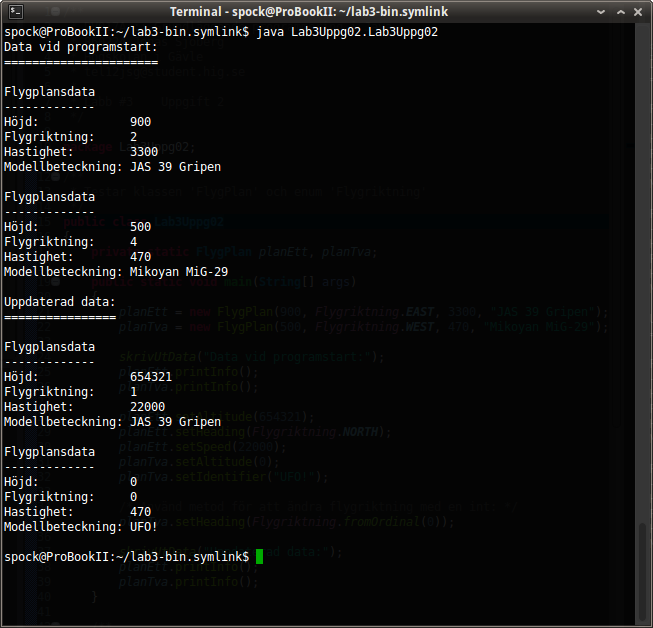
\includegraphics[width=\linewidth]{img/02.png}
    \caption{Körning av koden till Uppgift~\ref{sec:uppg02}}
    \label{fig:uppg02-screenshot}
\end{figure}


    \section{Uppgift 3}\label{sec:uppg03}

\subsection{Instruktioner}
\begin{verbatim}
3. Skriv en klass Cirkel som representerar en cirkel. I klassen ska följande
   två instansvariabler ingå:

   radie (int), färg (String)

   I parentes står lämplig datatyp.

   I klassen ska finnas en metod för var och en av följande operationer:

   - ändra färgen på cirkeln
   - returnera cirkelns färg
   - ändra cirkelns radie
   - returnera cirkelns radie
   - beräkna och returnera cirkelns omkrets
   - beräkna och returnera cirkelns area


   När man ska initiera ett cirkel-objekt ska man kunna välja på följande två
   alternativ:

   - välja *både* färg och radie på cirkeln
   - välja endast radien på cirkeln, men cirkelns färg blir alltid gul

   Detta betyder att du behöver två stycken konstruktorer (som överlagrar
   varandra) i din klass.

   Slutligen skriv ett testprogram som testar så att klassens metoder fungerar
   som de ska.  Skapa åtminstone två stycken cirkel-objekt, som använder sig av
   olika konstruktorer. Alla decimaltals-utskrifter på skärmen ska avrundas
   till *en* decimal.

   Tips: För att vid utskrift avrunda ett decimaltal använd klassen
   DecimalFormat, finns exempel i boken hur du använder denna. Den ligger i
   paketet java.text, du måste alltså importera denna klass i ditt testprogram.
\end{verbatim}


\subsection{Källkod}
\javacode{src/Lab3Uppg03/Lab3Uppg03.java}
\caption{Lab3Uppg03.java}
\label{src:uppg03}

\javacode{src/Lab3Uppg03/Cirkel.java}
\caption{Cirkel.java}
\label{src:cirkel}


\subsection{Skärmdump}
\begin{figure}[htbp]
    \centering
        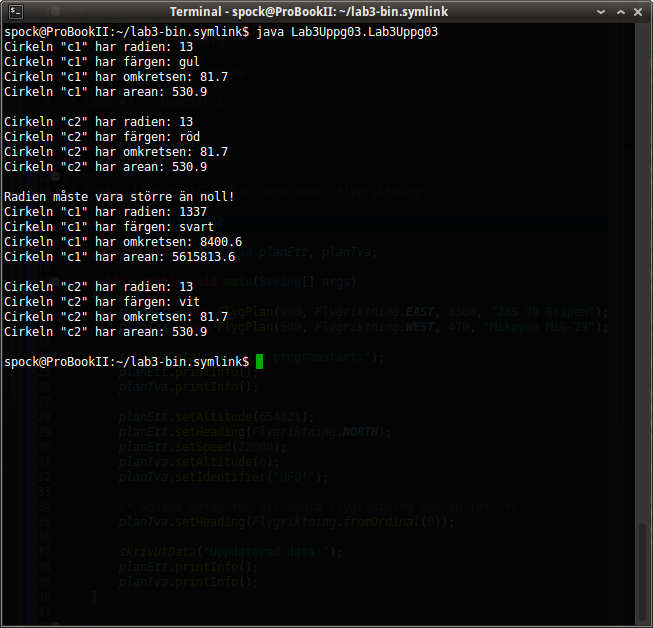
\includegraphics[width=\linewidth]{img/03.png}
    \caption{Körning av koden till Uppgift~\ref{sec:uppg03}}
    \label{fig:uppg03-screenshot}
\end{figure}


    \section{Uppgift 4}\label{sec:uppg04}

\subsection{Instruktioner}
Skriv en klass \texttt{Personbil} som representerar en personbil. Klassen ska
innehålla följande 4 instansvariabler. Välj själv passande datatyp:

\begin{itemize}
\itemsep1pt\parskip0pt\parsep0pt
\item bilmodell
\item årsmodell
\item registreringsnr
\item bilfärg
\end{itemize}

Det ska finnas metoder för var och en av följande operationer:

\begin{itemize}
\itemsep1pt\parskip0pt\parsep0pt
\item returnera bilens modell
\item returnera bilens årsmodell
\item returnera bilens regnr
\item ändra bilens färg
\item returnera bilens färg
\item skriva ut bilens samtliga data (metodens returtyp ska vara void)
\end{itemize}

Skriv sedan ett testprogram där du skapar 2 st personbils-objekt och sedan
testar samtliga metoder. Objektens instansvariabler ska via konstruktorn
initieras med följande värden:

\begin{verbatim}{\small}
Bil1 : bilmodell Saab, årsmodell -90, regnr CCC222 och färg röd.
Bil2 : bilmodell Volvo, årsmodell -99, regnr ABC988 och färg svart.
\end{verbatim}


\subsection{Kommentar}
Programmet \texttt{PersonbilGUI} skapades med verktyget \texttt{WindowBuilder}
i Eclipse Mars. Programmet visar hur typen \texttt{Color} kan användas i ett
GUI.  Metoden \texttt{toString()} används för att skriva ut färgen. Den visas
då i RGB-format. För att programmet ska skriva ut färgen som ett enkelt ord kan
en möjlig lösning nyttja en \texttt{enum} som "mappade" objekt av typen
\texttt{Color} med textsträngar av typen String. Typen kunde representera en
färg som sedan kan returneras i "fler former", t.ex. \texttt{Color} och
textsträng.
Referenser för \texttt{Color} och \texttt{Swing}:

\mbox{Color -- The Java Language Specification, Java SE 7 Edition}
\footnote{\url{http://docs.oracle.com/javase/7/docs/api/java/awt/Color.html}}

\mbox{Swing Tutorial -- The Java Tutorials}
\footnote{\url{http://docs.oracle.com/javase/tutorial/uiswing/}}


\subsection{Källkod}
\subsubsection{Lab3Uppg04.java}
\javacode{src/Lab3Uppg04/Lab3Uppg04.java}
\caption{Lab3Uppg04.java}
\label{src:uppg04}

\subsubsection{Personbil.java}
\javacode{src/Lab3Uppg04/Personbil.java}
\caption{Personbil.java}
\label{src:personbil}

\subsubsection{Personbil.java}
\javacode{src/Lab3Uppg04/PersonbilGUI.java}
\caption{PersonbilGUI.java}
\label{src:personbilgui}


\subsection{Skärmdump}
Se Figur~\ref{fig:uppg04-screenshot-cli} för skärmdump på körning av koden i 
Sektion~\ref{src:uppg04}.
\\
Figur~\ref{fig:uppg04-screenshot-gui1} och Figur~\ref{fig:uppg04-screenshot-gui2} 
visar körning av koden i Sektion~\ref{src:personbilgui}.

\begin{figure}[htbp]
    \centering
        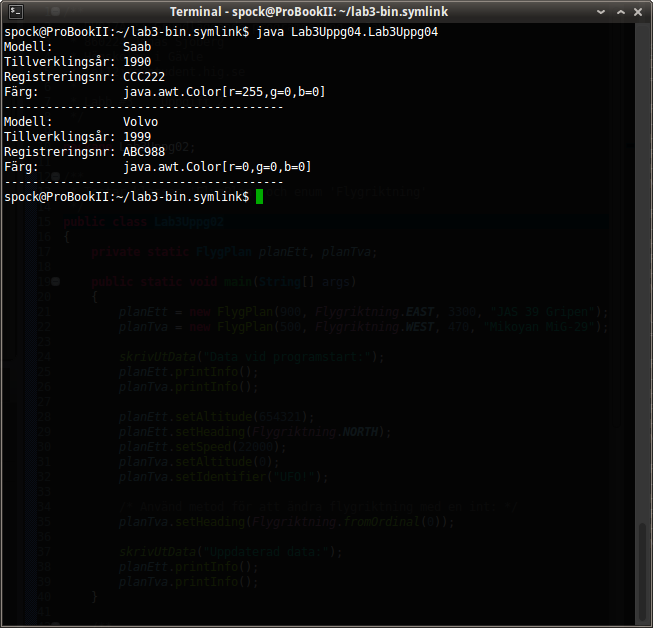
\includegraphics[width=\linewidth]{img/04.png}
    \caption{Körning av koden till Uppgift~\ref{sec:uppg04}}
    \label{fig:uppg04-screenshot-cli}
\end{figure}

\begin{figure}[htbp]
    \centering
        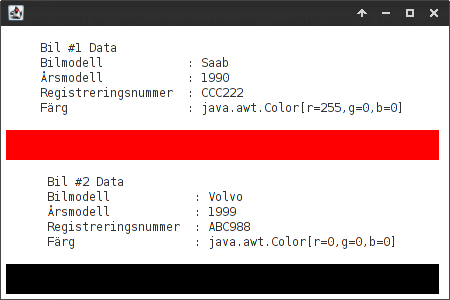
\includegraphics[width=0.75 \linewidth]{img/personbil-gui_1.png}
    \caption{Körning av \texttt{PersonbilGUI} från Uppgift~\ref{sec:uppg04}}
    \label{fig:uppg04-screenshot-gui1}
\end{figure}

\begin{figure}[htbp]
    \centering
        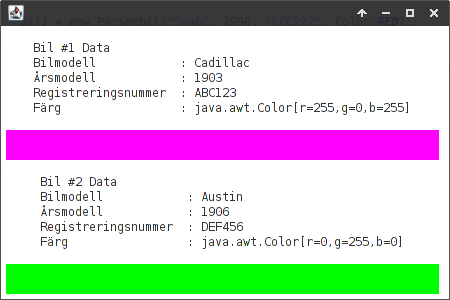
\includegraphics[width=0.75 \linewidth]{img/personbil-gui_2.png}
    \caption{Körning av \texttt{PersonbilGUI} från Uppgift~\ref{sec:uppg04} med andra bilar}}
    \label{fig:uppg04-screenshot-gui2}
\end{figure}


    \section{Uppgift 5}\label{sec:uppg05}

\subsection{Instruktioner}
\begin{Verbatim}[fontsize=small]
Skriv en klass Bilagare som representerar en bilägare. Klassen ska ha följande
tre instansvariabler:

namn (String), adress (String), bil (Personbil)

Instansvariablernas typer står inom parentes. I denna uppgift ska du även
använda dig av klassen Personbil som du skapade i uppgift 4. Efterson en
bilägare äger en bil så måste vi ha med instansvariabeln bil, som är en
referens till ett objekt av klassen Personbil.

I klassen Bilagare ska det finnas metoder för var och en av följande
operationer:

- returnera bilägarens namn
- returnera bilagarens adress
- bilägaren säljer sin bil (sätt instansvariabeln bil att ha värdet null)
- bilägaren köper ny bil (skicka som parameter med referensen till detta
  bil-objekt)
- skriv ut alla data om bilägarens bil, om han inte äger nån bil så ska
  valfritt meddelande (t.ex "Äger ingen bil för närvarande") istället
  skrivas ut. Metoden ska ha returtypen void.
- skriv ut bilägarens namn och adress.

Det ska naturligtvis finnas en konstruktor så att du kan initiera de tre
instansvariablerna.

Skriv ett testprogram som utför följande:

- Skapa två Personbils-objekt. Initiera objekten med valfria värden.
- Skapa ett Bilägare-objekt. Initiera objektet med valfria värden, ägarens
  bil måste dock vara någon av de två personbils-objekten.
- Skriv ut bilägarens namn och adress.
- Skriv ut data om bilägarens bil.
- Bilägaren säljer sin bil.
- Skriv ut data om bilägarens bil.
- Bilägaren köper en bil. Låt honom köpa någon av de två skapade
  personbils-objekten.
- Skriv ut data om bilägarens bil.
\end{Verbatim}


\subsection{Källkod}
\subsubsection{Lab3Uppg05.java}
\javacode{src/Lab3Uppg05/Lab3Uppg05.java}
\caption{Lab3Uppg05.java}
\label{src:uppg05}

\subsubsection{Bilagare.java}
\javacode{src/Lab3Uppg05/Bilagare.java}
\caption{Bilagare.java}
\label{src:bilagare}


\subsection{Skärmdump}
Se Figur~\ref{fig:uppg05-screenshot} för skärmdump på körning av koden i 
Sektion~\ref{src:uppg05}.

\begin{figure}[htbp]
    \centering
        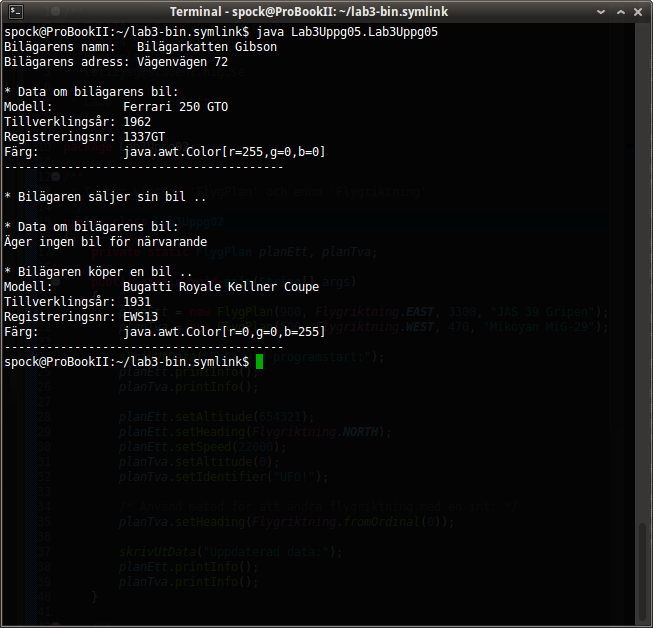
\includegraphics[width=\linewidth]{img/05.png}
    \caption{Körning av koden till Uppgift~\ref{sec:uppg05}}
    \label{fig:uppg05-screenshot}
\end{figure}


    \section{Uppgift 6}\label{sec:uppg06}

\subsection{Instruktioner}
\begin{Verbatim}[fontsize=\small]
Skriv en klass som heter Berakning. Klassen ska användas för olika beräkningar
med tre stycken valfria heltal. Klassen innehåller inga instansvariabler.

De operationer (beräkningar) som klassen ska kunna utföra är följande:

- Beräkna och returnera summan av tre stycken heltal. Talen kommer in via
  parametrar.
- Beräkna och returnera produkten av tre stycken heltal. Talen kommer in via
  parametrar.
- Beräkna och returnera det minsta av tre stycken heltal. Talen kommer in
  via parametrar.
- Beräkna och returnera det största av tre stycken heltal. Talen kommer in
  via parametrar.

Skriv sedan ett program som beräknar och skriver ut summan resp produkten av
talen 4, 8 och 78. Och som sedan skriver ut det minsta och största talet av
talen 100, 23 och 27. Du ska använda dig av metoderna i klassen Berakning för
att utföra dessa beräkningar!
\end{Verbatim}


\subsection{Källkod}
\subsubsection{Lab3Uppg06.java}
\javacode{src/Lab3Uppg06/Lab3Uppg06.java}
\caption{Lab3Uppg06.java}
\label{src:uppg06}

\subsubsection{Berakning.java}
\javacode{src/Lab3Uppg06/Berakning.java}
\caption{Berakning.java}
\label{src:berakning}


\subsection{Skärmdump}
Se Figur~\ref{fig:uppg06-screenshot} för skärmdump på körning av koden i
Sektion~\ref{src:uppg06}.

\begin{figure}[htbp]
    \centering
        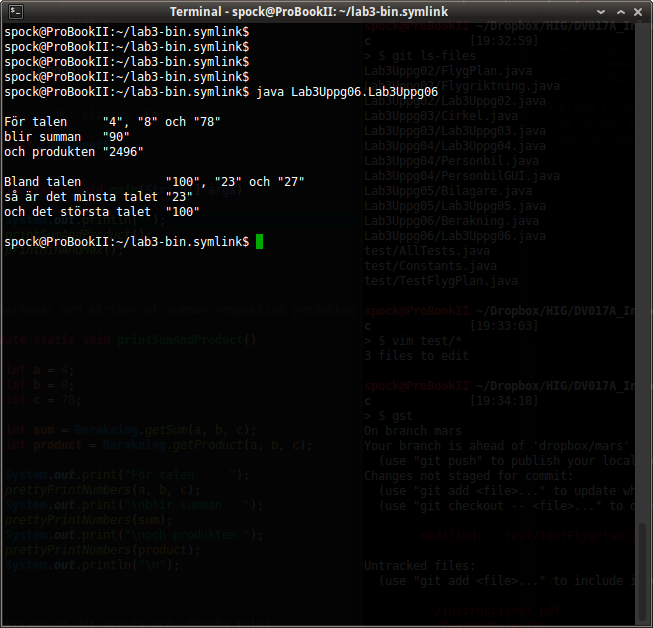
\includegraphics[width=\linewidth]{img/06.png}
    \caption{Körning av koden till Uppgift~\ref{sec:uppg06}}
    \label{fig:uppg06-screenshot}
\end{figure}



\end{document}
